\documentclass[a4paper, 11pt, final, garamond]{book}
\usepackage{cours-preambule}

\makeatletter
\renewcommand{\@chapapp}{Devoir surveill\'e -- num\'ero}
\makeatother

\begin{document}
\setcounter{chapter}{1}

\def\lspace{25}

\chapter{Commentaires sur le DS \oldno02}

\section{Commentaires généraux}


% \begin{tcb}[bld,cnt,fontupper=\Large](impo){Points clés}
% 	\begin{itemize}
% 		\item Les interrupteurs, ouverts ou fermés, ne sont PAS des résistances~!
% 		\item Interrupteur fermé (fil) $\Ra i \neq 0, u = 0$~;
% 		\item Interrupteur ouvert $\Ra i=0, u \neq 0$~!
% 		\item Condition initiale $\cancel{\Lra}$ en $t=0$, mais en $t$ initial~!
% 	\end{itemize}
% \end{tcb}

\textbf{Les tensions ne sont pas des vecteurs~!!}

\begin{center}
	\fatbox{%
		\large \bfseries
		ARRÊTEZ AVEC LES $\times$ QUI RESSEMBLENT À DES $+$~!!
	}%
\end{center}
Arrêtez avec les $\times$ tout court~! Pour la peine, nouveau malus $-X$.


% \begin{center}
% 	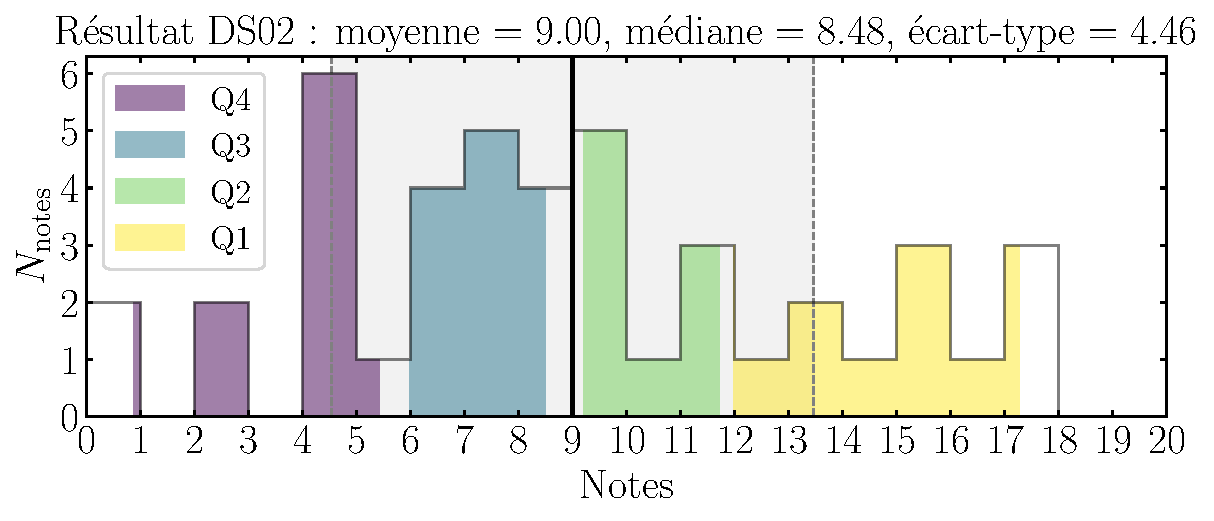
\includegraphics[width=.7\linewidth]{DS02_rslt.pdf}
% \end{center}

\setcounter{section}{0}
\section[24]"E"{Circuit de résistances}

C'est intolérable de ne pas refaire de schémas. Il va falloir vraiment
travailler le fait de faire des schémas tout le temps, toute l'année, pour tout,
pour toujours.

\begin{enumerate}[label=\sqenumi]
	\item[n]{5}% Q1
	      Bien.
	\item[n]{4}% Q2
	      Pas trop de problèmes d'inhomogénéité, bravo~! Par contre, \textbf{faites le
		      schéma équivalent}.
	\item[n]{4}% Q3
	      Idem, schémas équivalents.
	\item{}[\fbox{4-5}] % Q4-5
	      Il \textbf{faut} voir les PdT et PdC. Entraînez-vous à les identifier.
	      \textbf{Beaucoup de problèmes de signes} à cause du fléchage. Il faut savoir
	      revenir exactement à la situation du cours~!
	      \smallbreak
	      Vous ne pouvez pas trouvé un $I_k > I\ind{para}$, par définition du
	      \textbf{diviseur} de courant~!

\end{enumerate}

\setcounter{section}{0}
\section[47]"P"{Alimentation d'un train}
\begin{enumerate}[label=\sqenumi]
	\item[n]{3}% Q1
	      Bien.
	\item[n]{2}% Q2
	      Bien.
	\item[n]{5}% Q3
	      \textbf{Il faut \xul{choisir} la bonne valeur} dans le résultat d'un
	      trinôme~! À la fin, il n'y a bien qu'une seule tension…
	\item[n]{4}% Q4
	\item[n]{3}% Q5
	\item[n]{3}% Q6
	\item[n]{2}% Q7
	\item[n]{4}% Q8
	\item[n]{6}% Q9
	      Revenez à la définition des générateurs en les séparant~: ici, en séparent
	      les générateur de \textsc{Thévenin} de gauche, $R_{c_1}$ et $R_{r_1}$ sont
	      en série~!
	\item[n]{7}% Q10
	\item[n]{2}% Q11
	\item[n]{4}% Q12
	\item[n]{2}% Q13
\end{enumerate}

\section[68]"P"{Étude d'une lampe de secours rechargeable}
\begin{enumerate}[label=\sqenumi]
	\item[n]{10}% Q1
	      \vspace{-22pt}
	      \begin{itemize}
		      \item \textbf{RCT convention générateur}~!! Ça doit vous \textbf{choquer}
		            d'avoir un signe $-$ devant l'ordre 0. Ça nous donnerait une
		            exponentielle qui diverge en $t \to \infty$~!
		      \item Par continuité de la tension \textbf{aux bornes de $C$}~!
	      \end{itemize}
	\item[n]{3}% Q2
	\item[n]{4}% Q3
	\item[n]{14}% Q4
	\item[n]{6}% Q5
	\item[n]{8}% Q6
	\item[n]{7}% Q7
	\item[n]{6}% Q8
	\item[n]{7}% Q9
	\item[n]{3}% Q10
\end{enumerate}

\section[71]"P"{Guirlandes électriques}
\begin{enumerate}[label=\sqenumi]
	\item[n]{2}% Q1
	\item[n]{6}% Q2
	\item[n]{5}% Q3
	\item[n]{3}% Q4
	\item[n]{2}% Q5
	\item[n]{3}% Q6
	\item[n]{3}% Q7
	\item[n]{2}% Q8
	\item[n]{3}% Q9
	\item[n]{5}% Q10
	\item[n]{5}% Q11
	\item[n]{8}% Q12
	\item[n]{7}% Q13
	\item[n]{6}% Q14
	\item[n]{2}% Q15
	\item[n]{5}% Q16
	\item[n]{2}% Q17
	\item[n]{2}% Q18
\end{enumerate}

\end{document}
